\documentclass{beamer}
\usepackage{listings}
\usepackage[outdir=./images/]{epstopdf}
\definecolor{codegreen}{rgb}{0,0.6,0}
\definecolor{codegray}{rgb}{0.5,0.5,0.5}
\definecolor{codepurple}{rgb}{0.58,0,0.82}
\definecolor{backcolour}{rgb}{0.95,0.95,0.92}


\lstdefinestyle{mystyle}{
	backgroundcolor=\color{backcolour},
	commentstyle=\color{codegreen},
	keywordstyle=\color{magenta},
	numberstyle=\tiny\color{codegray},
	stringstyle=\color{codepurple},
	basicstyle=\ttfamily\footnotesize,
	breakatwhitespace=false,
	breaklines=true,
	captionpos=b,
	keepspaces=true,
	numbers=left,
	numbersep=5pt,
	showspaces=false,
	showstringspaces=false,
	showtabs=false,
	tabsize=2
}
\lstset{style=mystyle}


\usetheme{Frankfurt}
\beamertemplatenavigationsymbolsempty

\title{JaxFlowSim}

\author{Diego Renner}

\begin{document}

\section{Introduction}
\maketitle

\begin{frame}
	\frametitle{What}
	\begin{block}{What is jaxFlowSim?}
		\begin{itemize}
			\item 1D-haemodynamics solver
			\item written in JAX
			\item differentiable
		\end{itemize}
	\end{block}
	\vspace{5mm}
\end{frame}

\begin{frame}
	\frametitle{Why}
	\begin{block}{Motivation}
		\begin{itemize}
			\item towards personalised medicine
			\item parameter inference
			\item sensitivity analysis
		\end{itemize}
	\end{block}
	\vspace{5mm}
\end{frame}


\section{Code}

\begin{frame} [fragile]
	\frametitle{Code Structure}
	\begin{lstlisting}[basicstyle=\fontsize{8}{8}\selectfont\ttfamily, language=Python, caption=The code structure of an entire simulation is given here in pseudocode. Each line is detailed throughout this section., label=lst:pc, escapechar=|] 
		def runSimulation(config_filename, J) 
			config = loadConfig(config_filename) |\label{ln:init_start}|
			simulation_data = buildArterialNetwork(config) |\label{ln:init_end}|

			P_t = [0] |\label{ln:pt}|

			converged = False |\label{ln:whout1}|
			while not converged: |\label{ln:whout2}|
				t = 0 |\label{ln:t0}|
				i = 0 |\label{ln:i0}|
				P_t_temp = P_t |\label{ln:cp}|
				while t < T:
					dt = computeDt(simulation_data) |\label{ln:cfl}|
					simulation_data = setBoundaryValues(simulation_data, dt) |\label{ln:bv    }|
					simulation_data = muscl(simulation_data, dt) |\label{ln:muscl}|
					P_t[i,:] = savePressure(simulation_data) |\label{ln:svp}|
					t = t + dt |\label{ln:updt}|
					i = i + 1 |\label{ln:updi}|
					if i >= J:
						break
				converged = checkConv(P_t, P_t_temp) |\label{ln:conv}|
\end{lstlisting}
\end{frame}
\begin{frame}
	\frametitle{Padding}
	without padding
	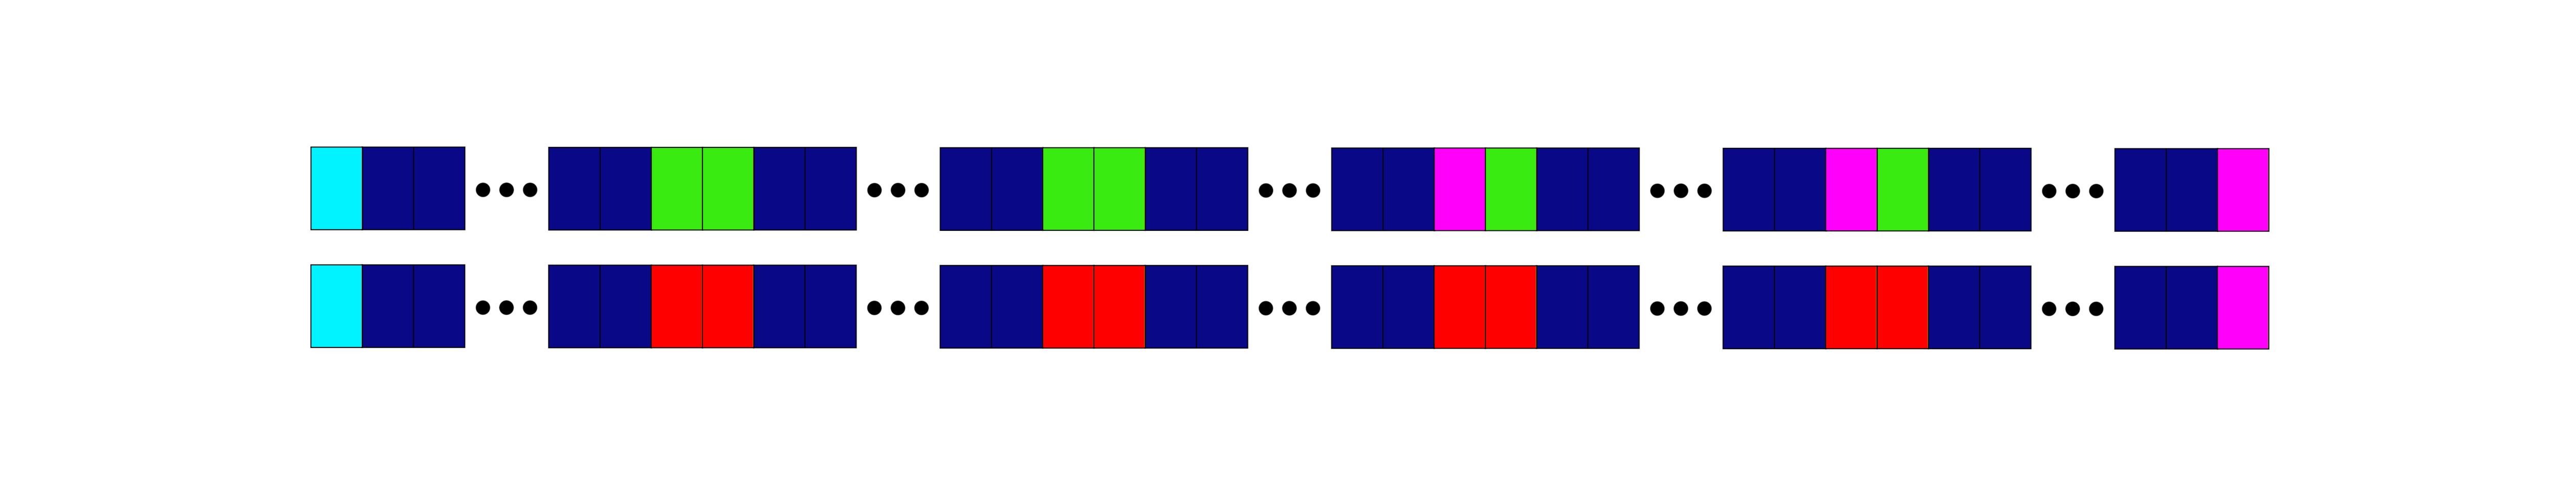
\includegraphics[width=\textwidth]{images/padding1.eps}
	with padding
	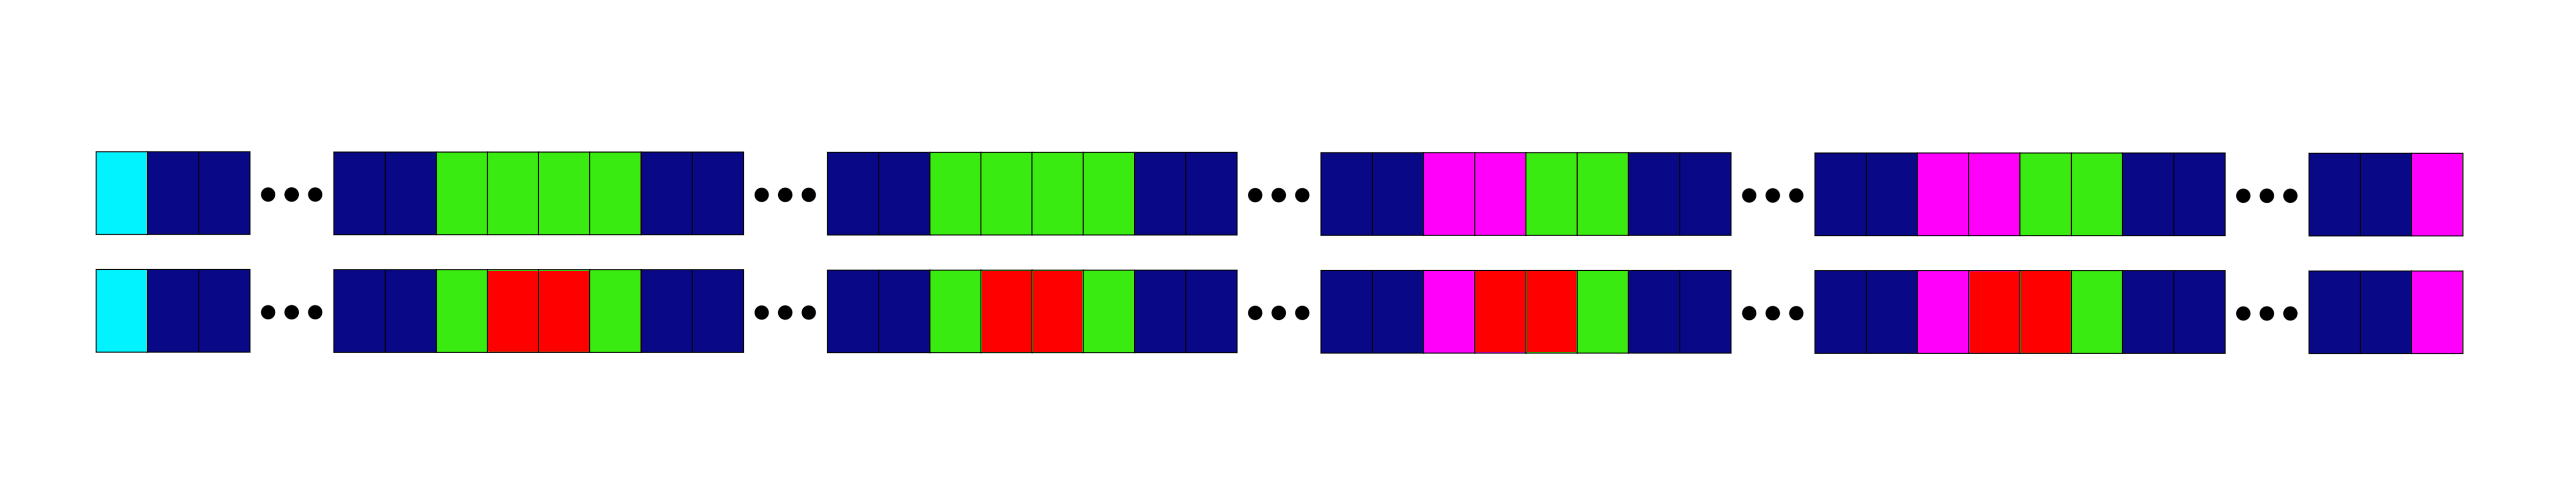
\includegraphics[width=\textwidth]{images/padding2.eps}
\end{frame}
\begin{frame}
	\frametitle{Masking}
	\includegraphics[width=\textwidth]{images/masking.eps}
\end{frame}

\section{Results}
\begin{frame}
	\frametitle{Validation}
	\begin{figure} [H]
		\centering
		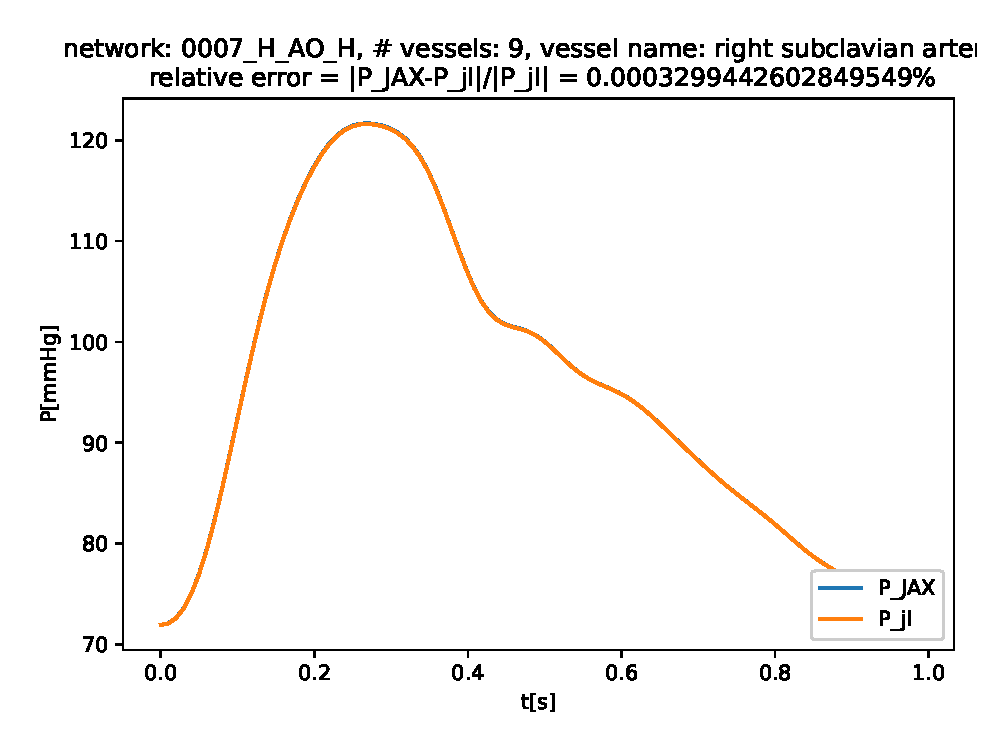
\includegraphics[width=0.33\columnwidth]{images/0007_H_AO_H_right_subclavian_artery_P.eps}
		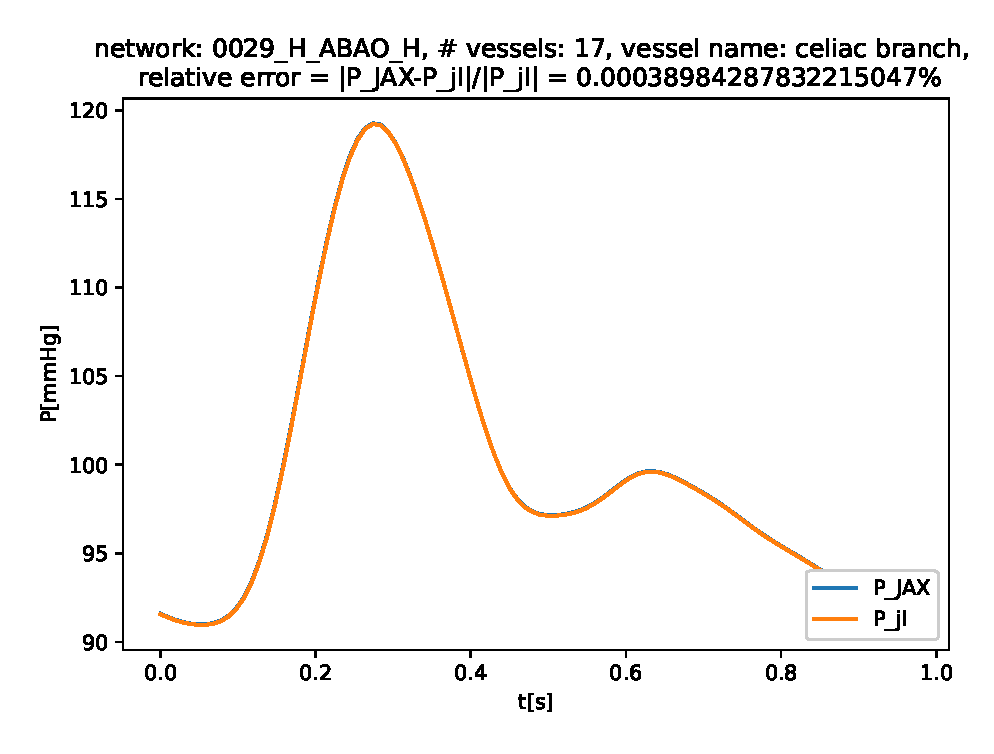
\includegraphics[width=0.33\columnwidth]{images/0029_H_ABAO_H_celiac_branch_P.eps
		}
		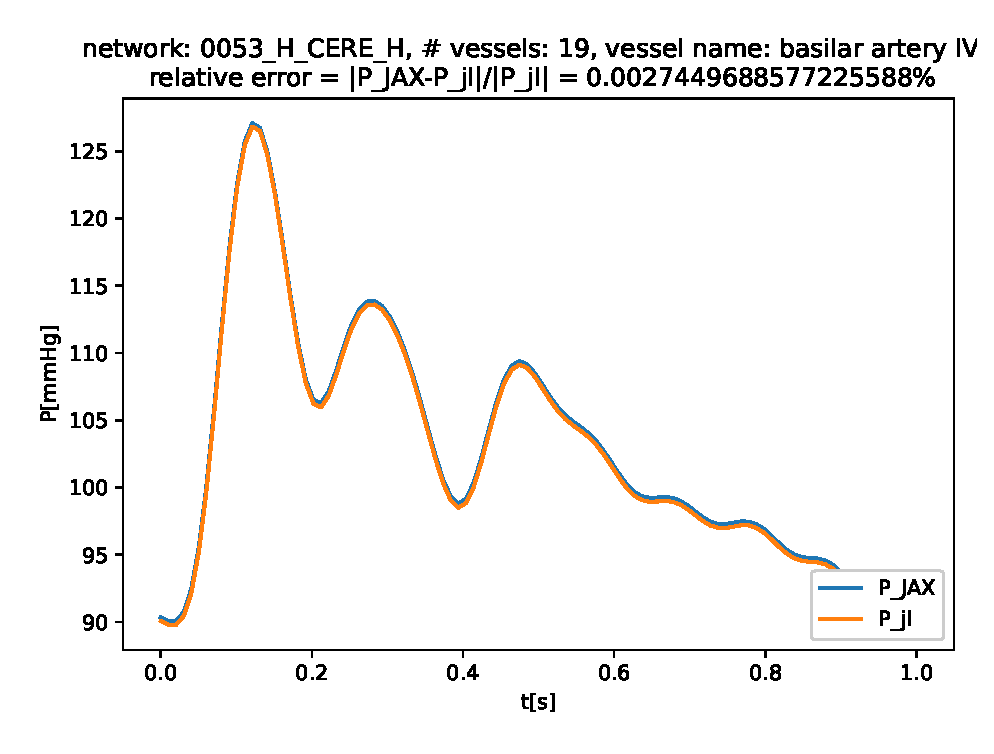
\includegraphics[width=0.33\columnwidth]{images/0053_H_CERE_H_basilar_artery_IV_P.eps}
		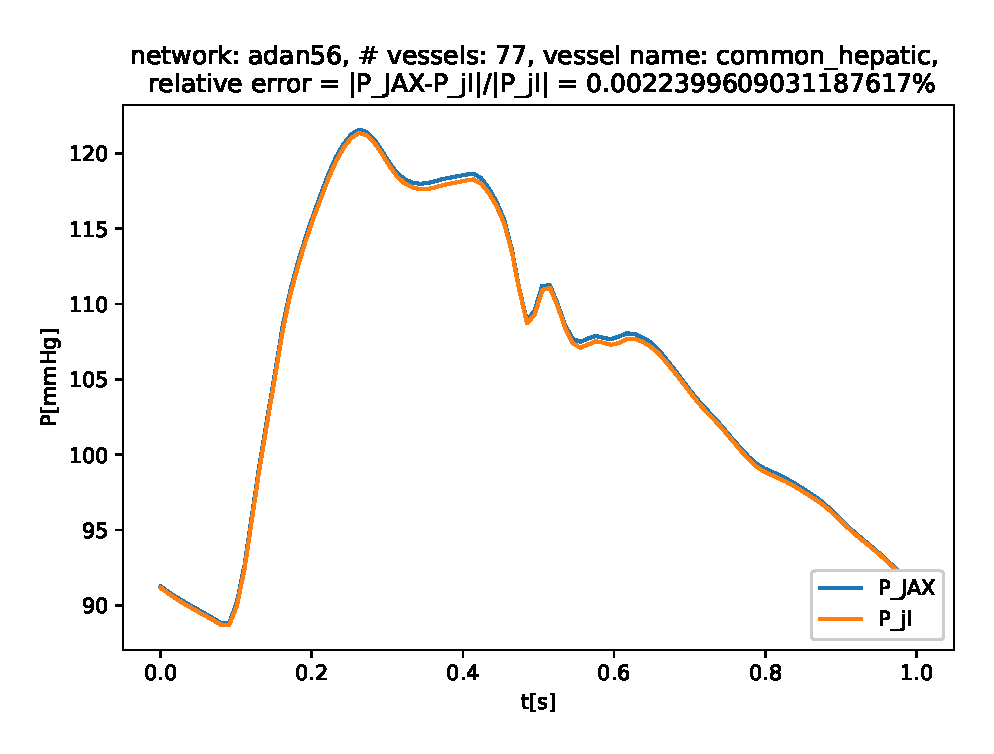
\includegraphics[width=0.33\columnwidth]{images/adan56_common_hepatic_P.eps}
		\caption{Our code and the openBF code produce close
		to the same output.
	In the 0007\_H\_AO\_H and the 0029\_H\_ABAO\_H networks this even leads to the plot of the data from our code being almost completely obfuscated by the openBF data.}
		\label{fig:val}
	\end{figure}
\end{frame}
\begin{frame}
	\frametitle{Comparison}
\begin{figure} [H]
    \centering
    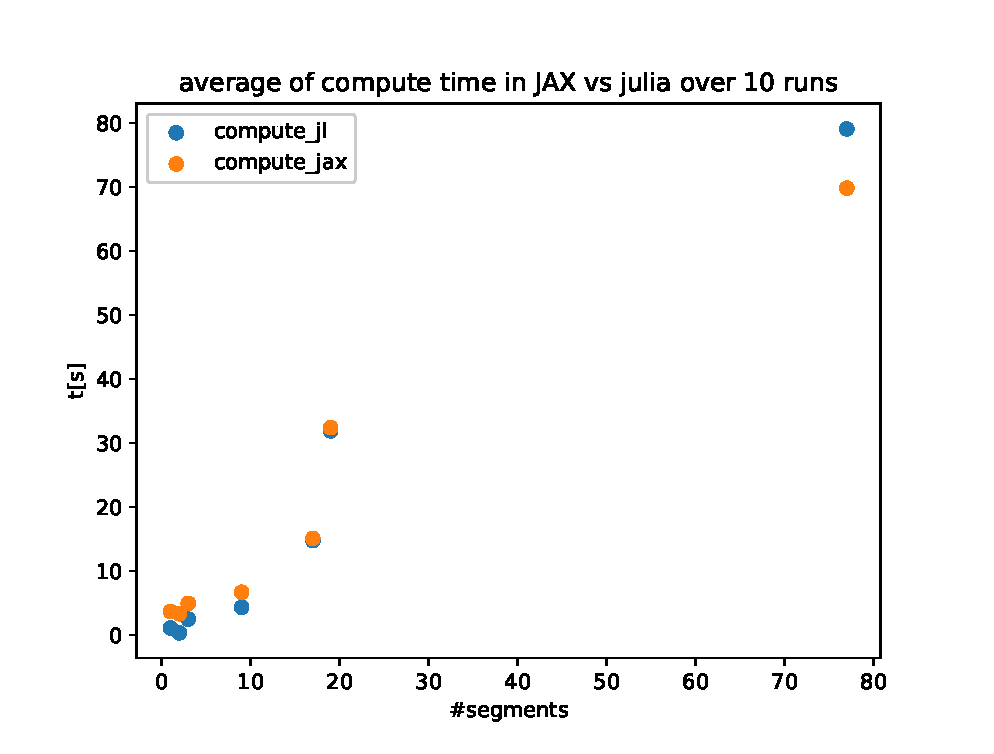
\includegraphics[width=0.7\columnwidth]{images/comparison.eps}
    \caption{Smaller systems suffer from the overhead JAX compilation creates but
for larger models the execution times become equal. For the largest model the JAX
code even beats the julia implementation.}
    \label{fig:comparison}
\end{figure}

\end{frame}
\begin{frame}
	\frametitle{Inference}
	\begin{block}{Demo}
		inferring an outlet resistance parameter from precomputed data
	\end{block}
\end{frame}

\section{Future Work}
\begin{frame}
	\frametitle{Points of interest}
	\begin{block}{Motivation}
		\begin{itemize}
			\item improving performance (GPU optimization)
			\item fine tuning parameter inference
			\item sensitivity analysis
		\end{itemize}
	\end{block}
	\vspace{5mm}
\end{frame}

\begin{frame}
	\frametitle{Questions?}
	Thank you for your attention!
\end{frame}

\end{document}
